\chapter{Literature}
\label{ch:Literature}



\section{Literature Overview}
%-------------------------------------------%

In {\it Towards Integrated Imitation of Strategic Planning and Motion Modeling in Interactive Computer Games}, Dublin City University researchers Bernard Gorman and Mark Humphrys use imitation learning techniques to train an artificial agent to collect items in {\it Quake II} \cite{Gorman:2006}. Specifically, their agent must traverse three-dimensional environments in order to intelligently seek out desirable items, such as power-ups, weapons, and health pickups. Furthermore, the researchers set an additional requirement: the agent must ``employ human-like motion,'' which is to say that it must traverse the map in such a way that its movements appear fluid and natural, as if a human were controlling it rather than a machine. The researchers refer to this ``imitation of the player's movement'' as {\it motion modeling}. Gorman and Humphrys create their training dataset by retrieving state information from demo files. Specifically, they use topology learning techniques to define a Markov Decision Process or MDP based on all of the player and item positions noted in the demo. They then employ value iteration using information about the player's status, such as current health and inventory contents; this information is also derived from the demo. Value iteration assigns a utility to each state in the MDP and, ultimately, allows the agent to make decisions about where to travel next. Gorman and Humphrys also discuss their approach for motion modeling. First, they define a set of {\it action primitives} by reading all of the input data from the demo file and then disassociating that data from its context. This allows the agent to, after deciding where to navigate, lay out a series of {\it action primitives} which will allow it to reach its goal \cite{Gorman:2006}.

Gorman and Humphrys cite {\it Learning human-like Movement Behavior for Computer Games} by Christian Thurau and Christian Bauckhage of Bielefeld University. The paper describes an experimental study which provides a useful behavioral model while also challenging the conventional approach for developing videogame AI \cite{Thurau:2004}. Thurau and Bauckhage define a hierarchy of behavior types, consisting of reactive, tactical, and strategic behaviors. Strategic behaviors are essentially long-term plans for winning the game, such as which objectives to target and in what order. Contrast this with reactive behaviors, which are atomic, immediate decisions, such as moving in a particular direction, turning around, or firing a weapon. Tactical behaviors sit in between reactive and strategic, representing small-scale decisions such as circle-strafing an opponent, or choosing to run away from a battle in order to look for a health pickup \cite{Gorman:2006}. To implement an agent that demonstrates such behaviors, Thurau and Bauckhage employ topology learning techniques to train a type of neural network called a {\it neural gas}, using player position data extracted from demo files. This methodology should sound familiar; Gorman and Humphrys use some of the techniques which Thurau and Bauckhage discuss \cite{Thurau:2004}.

The research described heretofore addresses considerably more complex problems than the one this project seeks to solve, simply by virtue of their game environment being three rather than two-dimensional. Nonetheless, the problems are still very similar, and as such the solutions may also bear some resemblance as well. For one: {\it Rivals of Aether} replays and {\it Quake} demos provide the same kind of information. Furthermore, these projects, like our own, are seeking to create AI opponents that behave like human players. One could therefore reasonably wonder whether or not the techniques described above could translate into a two-dimensional space.

In {\it Learning to Act by Predicting the Future}, Cornell University researchers Alexey Dosovitskiy and Vladlen Koltun use supervised learning techniques to train an agent to play competitive deathmatches in {\it Doom} \cite{VDComp:2016}. Dosovitskiy and Koltun do so by using two distinctive data streams: one is high-dimensional and consists of ``raw visual, auditory, and tactile input,'' while the other is low-dimensional and provides basic game state information such as ``health, ammunition levels, and the number of adversaries overcome.'' These data streams are referred to as the {\it sensory} and {\it measurement} streams, and together they serve as inputs for a supervised learning model \cite{Dosovitskiy:2016}. The resulting AI, named IntelAct, performed remarkably well in the full deathmatch track of 2016 {\it Visual Doom} AI Competition \cite{VDComp:2016}.

However, on the same track in the 2017 competition, IntelAct was beaten by two other AI, with YanShi and Arnold4 coming in second and first place, respectively \cite{VDComp:2017}. In {\it Arnold: An Autonomous Agent to play FPS Games}, Devendra Singh Chaplot and Guillaume Lample from Carnegie Mellon University describe their implementation, which consists of a pair of Deep Q-Networks working together in tandem. One of the networks is concerned with learning policies related to combat, while the other does the same for environmental navigation. Champlot and Lample implement this model with {\it UltraDeep} and {\it Theano}. The result of their project is an AI that ``outperforms average humans as well as in-built game bots,'' which earned ``the highest kill-to-death ratio in both tracks of the Visual Doom AI Competition'' in 2017. Overall, this paper provides a convenient overview of the project \cite{Chaplot}. However, Chaplot and Lample go into far greater detail in the paper titled {\it Playing FPS Games with Deep Reinforcement Learning} \cite{Chaplot:2016}.

The results of Arnold and IntelAct deserve considerable attention, because their creators not only implemented creative solutions, but they also outperformed all of the other AIs during the 2017 and 2016 competitions. One notable common thread between the two projects is that the researchers found ways to break the problem into smaller, more manageable pieces. Chaplot and Lample do this at the learning stage by implementing two deep reinforcement learning networks \cite{Chaplot}, while Dosovitskiy and Koltun work from the input stage with their dual-stream approach \cite{Dosovitskiy:2016}.

In {\it Novel Moving Target Search Algorithms}, Peter K. K. Loh from Nanyang Technological University and Edmond C. Prakash from Manchester Metropolitan University explain the complexity behind creating an AI that can quickly and effectively respond to a human player's constantly changing position \cite{Loh:2009}. They state that this criteria creates conflicting requirements. They then introduce two Moving Target Search or MTS algorithms, called Fuzzy MTS and Abstraction MTS. These algorithms were compared against other MTS algorithms with promising results even within large problem spaces. \cite{Loh:2009}. Although the name "moving target search" might, in some contexts, sound like it is related to aiming a weapon and pointing it towards a so-called "moving target," that does not accurately describe what these algorithms are for. Rather, the the "moving target" in this case is meant in a more general sense. For example, in the IBM blog post titled {\it Solving AI’s moving-target search problem at IJCAI 2017}, an example of an MTS problem is given in the form of a cab trying to find a customer \cite{IBM:2017}. Thus, MTS algorithms may be a viable tool for our AI to employ.

In {\it ViZDoom: A Doom-based AI Research Platform for Visual Reinforcement}, Cornell University researchers Michal Kempa, Marek Wydmuch, Grzegorz Runc, Jakub Toczek, and Wojciech Jaśkowski discuss the benefits of their project, {\it ViZDoom}, as a research platform \cite{Kempka:2016}. They first discuss their earlier experiments with AI on the Atari 2600 that eventually led to the creation of {\it ViZDoom}. They also talk about the jump from two to three-dimensional environments. While this transition may seem problematic and difficult, in actuality a 3D space can simply be reinterpreted as an aggregation of many related 2D spaces. Kempa et all proceed to describe {\it ViZDoom} as a lightweight, fast and highly customizable framework for developing AI that plays {\it Doom}. As a proof-of-concept, the researchers implement and then train two bots using ``Q-Learning and convolutional deep neural networks.'' The result is two human-like AI that demonstrate not only how {\it ViZDoom} can serve as a useful tool for AI research, but also prove the viability of ``visual reinforcement learning in 3D realistic environments'' \cite{Kempka:2016}. This paper will serve as a valuable reference despite the difference in complexity between their problem and ours, because they are demonstrating the capabilities of the same machine learning algorithms which we are exploring.

In {\it Autoencoder-augmented Neuroevolution for Visual Doom Playing}, Cornell University researchers Samuel Alvernaz and Julian Togelius explore the use of an autoencoder alongside a neuroevolution technique called ``Covariance Matrix Adaptation Evolution Strategy'' or CMA-ES \cite{Alvernaz:2017}. An autoencoder is essentially a technique for simplifying and reconstructing images. The researchers implement their autoencoder using Keras, a high-level machine-learning library. They then use the autoencoder to generate a simplified version of the frame buffer to use as the input for their neural network, which they then train to complete health pack gathering exercises. The autoencoder's purpose is to convert a high-dimensional state space, that being the full-resolution frame buffer, into a comparatively low-dimensional substitute \cite{Alvernaz:2017}. The use of an autoencoder by Alvernaz et al can be directly compared with SethBling's use of simple downscaling and grayscaling. Both of these techniques result in a simplified state space; however, the key difference between them is that an autoencoder has the potential to learn a much more efficient way to achieve this goal. Otherwise, the one other key technique noted in this paper is CMA-ES. If our dataset, for whatever reason, proves insufficient or otherwise unusable, then neuroevolution algorithms such as this may be our best fall-back option.

%-------------------------------------------%



\section{Software}
%-------------------------------------------%

{\it SerpentAI} is an open source Python framework that allows researchers to write game agent scripts that have the ability to easily retrieve the frame buffer from any computer game and then send keyboard or controller input back to it. The framework is noteworthy for functioning entirely independently of the target game. Furthermore, it makes no presumptions about what machine learning techniques the user wants to implement and can support anything from simple reflex or random agents to the most advanced and cutting-edge neural networks \cite{SerpentAI}. Ergo, {\it SerpentAI} serves as a bridge between our artificial intelligence and its testing environment by providing a simple interface for retrieving frame buffer data from and sending control input to virtually any game runtime. This is achieved by writing a game agent program. Our game agent utilizes {\it TensorFlow}, which is self-described as ``an open source software library for numerical computation using data flow graphs,'' was designed explicitly for use in machine learning research, and is able to achieve exceptional performance by employing either GPU computation or SIMD CPU instruction set architectures, such as SSE \cite{TensorFlow}. However, our agent does not access {\it TensorFlow} directly. Rather, it uses {\it Keras}, a high-level machine-learning library designed to serve as an abstraction layer over foundational libraries like {\it TensorFlow}. The low-level library still performs all of the heavy-lifting; {\it Keras} simply removes some of the barriers to entry \cite{Keras}.

The target game for this project is {\it Rivals of Aether}. We selected {\it Rivals of Aether} because it supports the recording of replays, which are files that keep a record of what controller inputs were detected from which player during each frame of gameplay. Thus, whereas a conventional video recording associates each frame with its pixel data, a replay does so with each frame and its input data. This allows the game to simulate a past match in real-time with perfect accuracy by simply running a new match in which each player's control input is read from the replay file rather than from the controller.

\begin{figure}
	\caption{"Screenshot showing gameplay in Rivals of Aether"}
	\centering
	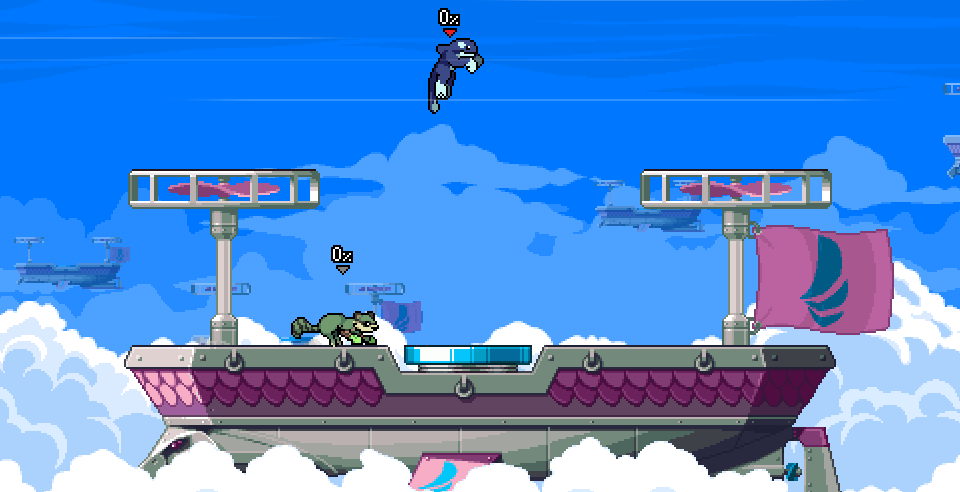
\includegraphics[scale = 0.5]{game.png} \\
\end{figure}

A replay file is therefore no different from a demo file from {\it Quake} or {\it Doom}. Such demos are often used in game-related machine learning research because a collection of demos is effectively a pre-labeled dataset. However, unlike {\it Doom} and {\it Quake}, which have websites such as {\it Speed Demo Archives} and {\it Quake Terminus}, {\it Rivals of Aether} does not have any well-established public repositories for replay files. Therefore, in order to build our collection of replays, we solicited from the {\it Rivals of Aether} community. Contributors provided us with a total of 1,020 replay files from a variety of settings, including tournaments, exhibitions, ranked matches, and private games. Adding our own personal replays brings the total up to 1,032. We plan on creating a program to simplify the replay files, as there is not currently any programs out there.

%-------------------------------------------%



\section{Other Sources}
%-------------------------------------------%

In {\it MariFlow - Self-Driving Mario Kart w/Recurrent Neural Network}, YouTuber SethBling trains a recurrent neural network to play Mario Kart using only the visual buffer \cite{SethBling:2017}. The goal of SethBling's project is to train the neural network to mimic the way he plays the game by having it learn from fifteen hours of his own recorded gameplay. The network, created in TensorFlow, receives ``a low-resolution grayscale version of the screen'' for input and employs multiple layers, sigmoid neurons, backpropagation, and ``long short term memory'' or LSTM cells in order to predict the appropriate controller action. Furthermore, SethBling runs ``interactive sessions'' in which he monitors the neural network while it plays the game so that he can identify situations in which it gets stuck; he then takes over control of the game so that he can show the neural network what to do in such situations. SethBling released several learning resources with his video, including his source code, utilities, and detailed instructions \cite{SethBling:2017}. Overall, not only does SethBling provide an excellent entry-level primer for the fundamentals of neural networks, he also gives an encouraging demonstration on how to solve a problem that is very close to our own.

%-------------------------------------------%